\begin{figure}[p]
\centering
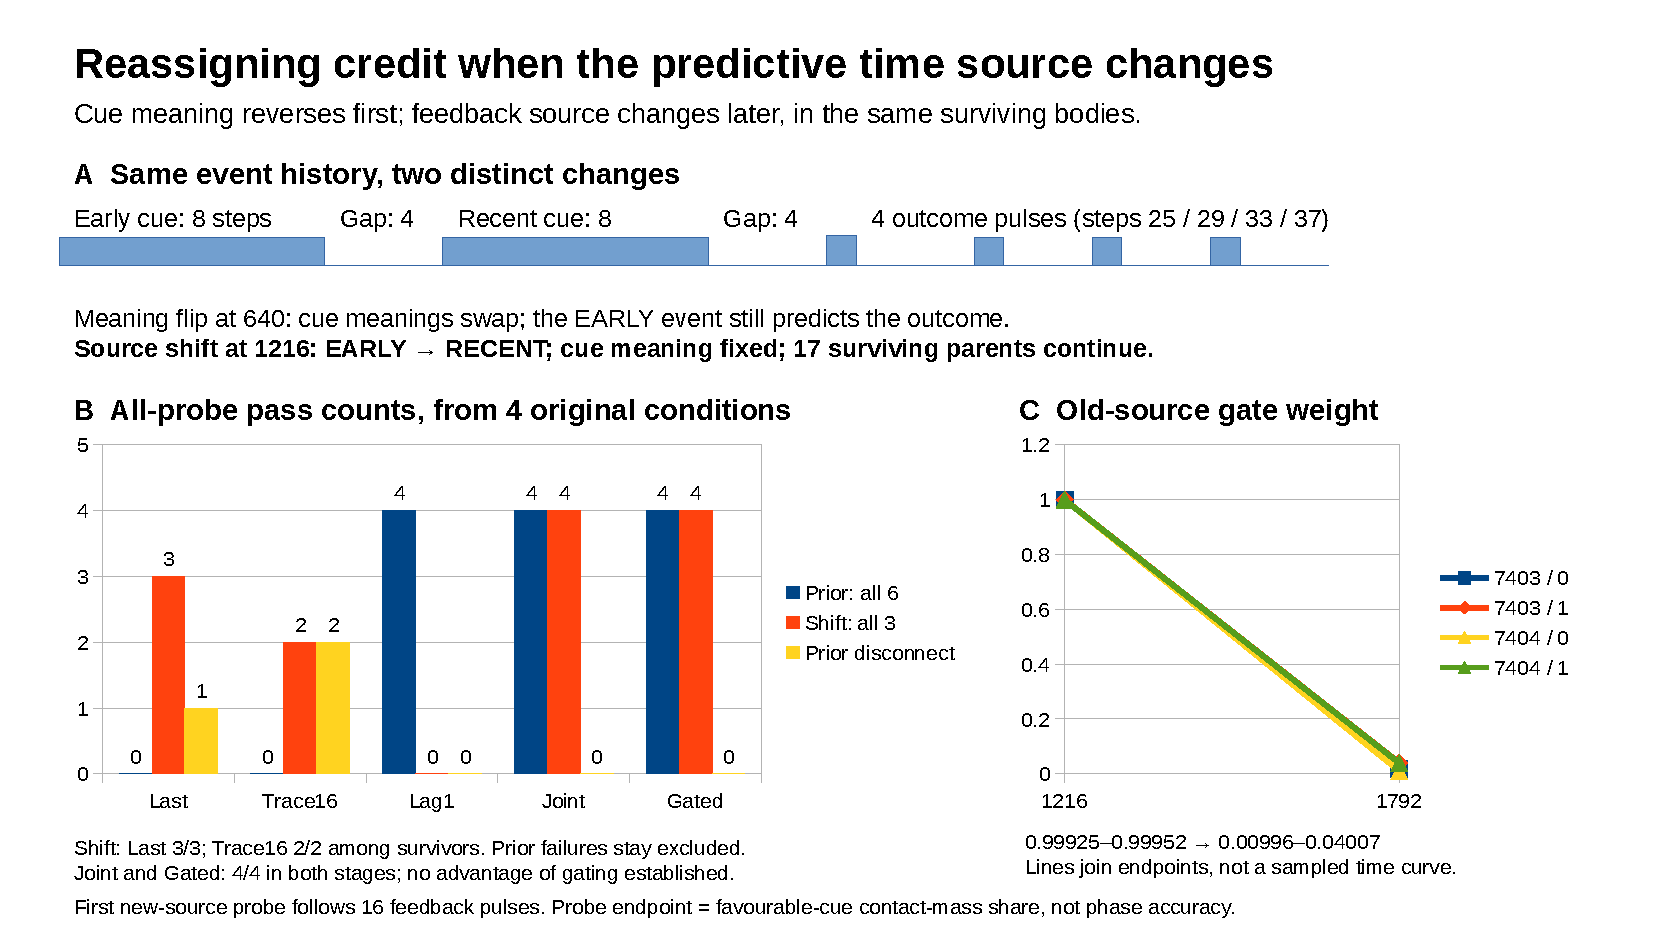
\includegraphics[width=\linewidth,height=.76\textheight,keepaspectratio]{work/longform_v047/figures/temporal_credit/temporal_credit.pdf}
\caption{\textbf{Useful history changes when the predictive temporal source changes.}
\textbf{A}, An independent intervening cue separates earlier from recent contact. The first change reverses cue meaning; the later change makes the recent event predictive while preserving cue meaning. Seventeen surviving bodies continue without reset. \textbf{B}, Fixed earlier-event delta, joint delta and gated experts pass all six initial acquisition, reversal and retention probes in four related seed--order conditions. Joint delta and gated experts also pass all three later probes in four of four conditions; fixed earlier-event delta fails a phase in all four. Earlier connectivity failures in recent-cue delta and the fixed trace remain failures. Their later three-of-three and two-of-two successes describe surviving subsets, shown relative to the original four-condition count. \textbf{C}, Individual gated-rule weights shift from the earlier to the recent source. Lines join the two measured endpoints and do not depict the intervening time course. Joint delta achieves the same behavioural coverage. Probe values are favourable-cue contact-mass fractions at the final frame; the first changed-source probe follows sixteen feedback pulses. These conservative bodies do not regenerate tissue, and additional learning arithmetic is not physically priced.}
\label{fig:temporal-credit}
\end{figure}
